
\begin{centering}

\huge{$\color{cyan}n^3\color{black}=$}
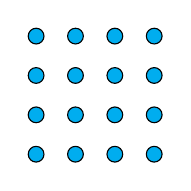
\begin{tikzpicture}
	\draw[fill=cyan] (0,0) circle [radius=0.1cm];
	\draw[fill=cyan] (0,0.5) circle [radius=0.1cm];
	\draw[fill=cyan] (0,1) circle [radius=0.1cm];
	\draw[fill=cyan] (0,1.5) circle [radius=0.1cm];
	
	\draw[fill=cyan] (0.5,0) circle [radius=0.1cm];
	\draw[fill=cyan] (0.5,0.5) circle [radius=0.1cm];
	\draw[fill=cyan] (0.5,1) circle [radius=0.1cm];
	\draw[fill=cyan] (0.5,1.5) circle [radius=0.1cm];
	
	\draw[fill=cyan] (1,0) circle [radius=0.1cm];
	\draw[fill=cyan] (1,0.5) circle [radius=0.1cm];
	\draw[fill=cyan] (1,1) circle [radius=0.1cm];
	\draw[fill=cyan] (1,1.5) circle [radius=0.1cm];
	
	\draw[fill=cyan] (1.5,0) circle [radius=0.1cm];
	\draw[fill=cyan] (1.5,0.5) circle [radius=0.1cm];
	\draw[fill=cyan] (1.5,1) circle [radius=0.1cm];
	\draw[fill=cyan] (1.5,1.5) circle [radius=0.1cm];
\end{tikzpicture}
\quad
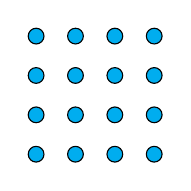
\begin{tikzpicture}
	\draw[fill=cyan] (0,0) circle [radius=0.1cm];
	\draw[fill=cyan] (0,0.5) circle [radius=0.1cm];
	\draw[fill=cyan] (0,1) circle [radius=0.1cm];
	\draw[fill=cyan] (0,1.5) circle [radius=0.1cm];
	
	\draw[fill=cyan] (0.5,0) circle [radius=0.1cm];
	\draw[fill=cyan] (0.5,0.5) circle [radius=0.1cm];
	\draw[fill=cyan] (0.5,1) circle [radius=0.1cm];
	\draw[fill=cyan] (0.5,1.5) circle [radius=0.1cm];
	
	\draw[fill=cyan] (1,0) circle [radius=0.1cm];
	\draw[fill=cyan] (1,0.5) circle [radius=0.1cm];
	\draw[fill=cyan] (1,1) circle [radius=0.1cm];
	\draw[fill=cyan] (1,1.5) circle [radius=0.1cm];
	
	\draw[fill=cyan] (1.5,0) circle [radius=0.1cm];
	\draw[fill=cyan] (1.5,0.5) circle [radius=0.1cm];
	\draw[fill=cyan] (1.5,1) circle [radius=0.1cm];
	\draw[fill=cyan] (1.5,1.5) circle [radius=0.1cm];
\end{tikzpicture}
\quad
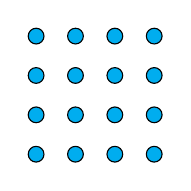
\begin{tikzpicture}
	\draw[fill=cyan] (0,0) circle [radius=0.1cm];
	\draw[fill=cyan] (0,0.5) circle [radius=0.1cm];
	\draw[fill=cyan] (0,1) circle [radius=0.1cm];
	\draw[fill=cyan] (0,1.5) circle [radius=0.1cm];
	
	\draw[fill=cyan] (0.5,0) circle [radius=0.1cm];
	\draw[fill=cyan] (0.5,0.5) circle [radius=0.1cm];
	\draw[fill=cyan] (0.5,1) circle [radius=0.1cm];
	\draw[fill=cyan] (0.5,1.5) circle [radius=0.1cm];
	
	\draw[fill=cyan] (1,0) circle [radius=0.1cm];
	\draw[fill=cyan] (1,0.5) circle [radius=0.1cm];
	\draw[fill=cyan] (1,1) circle [radius=0.1cm];
	\draw[fill=cyan] (1,1.5) circle [radius=0.1cm];
	
	\draw[fill=cyan] (1.5,0) circle [radius=0.1cm];
	\draw[fill=cyan] (1.5,0.5) circle [radius=0.1cm];
	\draw[fill=cyan] (1.5,1) circle [radius=0.1cm];
	\draw[fill=cyan] (1.5,1.5) circle [radius=0.1cm];
\end{tikzpicture}

\vspace{12pt}
\huge{$= \color{red}\tri{n}{3} \color{black}+ \color{green}? \color{black}= $}
\enspace
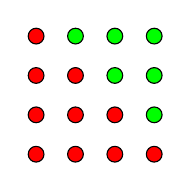
\begin{tikzpicture}
	\draw[fill=red] (0,0) circle [radius=0.1cm];
	\draw[fill=red] (0,0.5) circle [radius=0.1cm];
	\draw[fill=red] (0,1) circle [radius=0.1cm];
	\draw[fill=red] (0,1.5) circle [radius=0.1cm];
	
	\draw[fill=red] (0.5,0) circle [radius=0.1cm];
	\draw[fill=red] (0.5,0.5) circle [radius=0.1cm];
	\draw[fill=red] (0.5,1) circle [radius=0.1cm];
	\draw[fill=green] (0.5,1.5) circle [radius=0.1cm];
	
	\draw[fill=red] (1,0) circle [radius=0.1cm];
	\draw[fill=red] (1,0.5) circle [radius=0.1cm];
	\draw[fill=green] (1,1) circle [radius=0.1cm];
	\draw[fill=green] (1,1.5) circle [radius=0.1cm];
	
	\draw[fill=red] (1.5,0) circle [radius=0.1cm];
	\draw[fill=green] (1.5,0.5) circle [radius=0.1cm];
	\draw[fill=green] (1.5,1) circle [radius=0.1cm];
	\draw[fill=green] (1.5,1.5) circle [radius=0.1cm];
\end{tikzpicture}
\quad
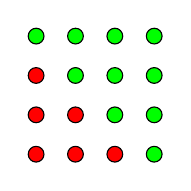
\begin{tikzpicture}

	\draw[fill=red] (0,0) circle [radius=0.1cm];
	\draw[fill=red] (0,0.5) circle [radius=0.1cm];
	\draw[fill=red] (0,1) circle [radius=0.1cm];
	\draw[fill=green] (0,1.5) circle [radius=0.1cm];
	
	\draw[fill=red] (0.5,0) circle [radius=0.1cm];
	\draw[fill=red] (0.5,0.5) circle [radius=0.1cm];
	\draw[fill=green] (0.5,1) circle [radius=0.1cm];
	\draw[fill=green] (0.5,1.5) circle [radius=0.1cm];
	
	\draw[fill=red] (1,0) circle [radius=0.1cm];
	\draw[fill=green] (1,0.5) circle [radius=0.1cm];
	\draw[fill=green] (1,1) circle [radius=0.1cm];
	\draw[fill=green] (1,1.5) circle [radius=0.1cm];
	
	\draw[fill=green] (1.5,0) circle [radius=0.1cm];
	\draw[fill=green] (1.5,0.5) circle [radius=0.1cm];
	\draw[fill=green] (1.5,1) circle [radius=0.1cm];
	\draw[fill=green] (1.5,1.5) circle [radius=0.1cm];
\end{tikzpicture}
\quad
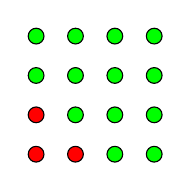
\begin{tikzpicture}
	\draw[fill=red] (0,0) circle [radius=0.1cm];
	\draw[fill=red] (0,0.5) circle [radius=0.1cm];
	\draw[fill=green] (0,1) circle [radius=0.1cm];
	\draw[fill=green] (0,1.5) circle [radius=0.1cm];
	
	\draw[fill=red] (0.5,0) circle [radius=0.1cm];
	\draw[fill=green] (0.5,0.5) circle [radius=0.1cm];
	\draw[fill=green] (0.5,1) circle [radius=0.1cm];
	\draw[fill=green] (0.5,1.5) circle [radius=0.1cm];
	
	\draw[fill=green] (1,0) circle [radius=0.1cm];
	\draw[fill=green] (1,0.5) circle [radius=0.1cm];
	\draw[fill=green] (1,1) circle [radius=0.1cm];
	\draw[fill=green] (1,1.5) circle [radius=0.1cm];
	
	\draw[fill=green] (1.5,0) circle [radius=0.1cm];
	\draw[fill=green] (1.5,0.5) circle [radius=0.1cm];
	\draw[fill=green] (1.5,1) circle [radius=0.1cm];
	\draw[fill=green] (1.5,1.5) circle [radius=0.1cm];
\end{tikzpicture}

\vspace{12pt}
\large{fill out \color{green}tetrahedral}
\quad

\begin{tikzpicture}
	\draw[fill=green] (1,1) circle [radius=0.1cm];
\end{tikzpicture}
\quad
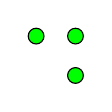
\begin{tikzpicture}
	\draw[fill=green] (0.5,0.5) circle [radius=0.1cm];
	\draw[fill=green] (0,0.5) circle [radius=0.1cm];
	\draw[fill=green] (0.5,0) circle [radius=0.1cm];
\end{tikzpicture}
\quad
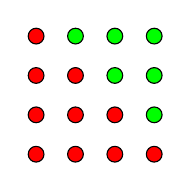
\begin{tikzpicture}
	\draw[fill=red] (0,0) circle [radius=0.1cm];
	\draw[fill=red] (0,0.5) circle [radius=0.1cm];
	\draw[fill=red] (0,1) circle [radius=0.1cm];
	\draw[fill=red] (0,1.5) circle [radius=0.1cm];
	
	\draw[fill=red] (0.5,0) circle [radius=0.1cm];
	\draw[fill=red] (0.5,0.5) circle [radius=0.1cm];
	\draw[fill=red] (0.5,1) circle [radius=0.1cm];
	\draw[fill=green] (0.5,1.5) circle [radius=0.1cm];
	
	\draw[fill=red] (1,0) circle [radius=0.1cm];
	\draw[fill=red] (1,0.5) circle [radius=0.1cm];
	\draw[fill=green] (1,1) circle [radius=0.1cm];
	\draw[fill=green] (1,1.5) circle [radius=0.1cm];
	
	\draw[fill=red] (1.5,0) circle [radius=0.1cm];
	\draw[fill=green] (1.5,0.5) circle [radius=0.1cm];
	\draw[fill=green] (1.5,1) circle [radius=0.1cm];
	\draw[fill=green] (1.5,1.5) circle [radius=0.1cm];
\end{tikzpicture}
\quad
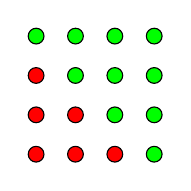
\begin{tikzpicture}

	\draw[fill=red] (0,0) circle [radius=0.1cm];
	\draw[fill=red] (0,0.5) circle [radius=0.1cm];
	\draw[fill=red] (0,1) circle [radius=0.1cm];
	\draw[fill=green] (0,1.5) circle [radius=0.1cm];
	
	\draw[fill=red] (0.5,0) circle [radius=0.1cm];
	\draw[fill=red] (0.5,0.5) circle [radius=0.1cm];
	\draw[fill=green] (0.5,1) circle [radius=0.1cm];
	\draw[fill=green] (0.5,1.5) circle [radius=0.1cm];
	
	\draw[fill=red] (1,0) circle [radius=0.1cm];
	\draw[fill=green] (1,0.5) circle [radius=0.1cm];
	\draw[fill=green] (1,1) circle [radius=0.1cm];
	\draw[fill=green] (1,1.5) circle [radius=0.1cm];
	
	\draw[fill=green] (1.5,0) circle [radius=0.1cm];
	\draw[fill=green] (1.5,0.5) circle [radius=0.1cm];
	\draw[fill=green] (1.5,1) circle [radius=0.1cm];
	\draw[fill=green] (1.5,1.5) circle [radius=0.1cm];
\end{tikzpicture}
\quad
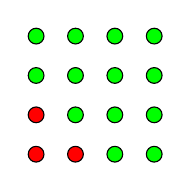
\begin{tikzpicture}
	\draw[fill=red] (0,0) circle [radius=0.1cm];
	\draw[fill=red] (0,0.5) circle [radius=0.1cm];
	\draw[fill=green] (0,1) circle [radius=0.1cm];
	\draw[fill=green] (0,1.5) circle [radius=0.1cm];
	
	\draw[fill=red] (0.5,0) circle [radius=0.1cm];
	\draw[fill=green] (0.5,0.5) circle [radius=0.1cm];
	\draw[fill=green] (0.5,1) circle [radius=0.1cm];
	\draw[fill=green] (0.5,1.5) circle [radius=0.1cm];
	
	\draw[fill=green] (1,0) circle [radius=0.1cm];
	\draw[fill=green] (1,0.5) circle [radius=0.1cm];
	\draw[fill=green] (1,1) circle [radius=0.1cm];
	\draw[fill=green] (1,1.5) circle [radius=0.1cm];
	
	\draw[fill=green] (1.5,0) circle [radius=0.1cm];
	\draw[fill=green] (1.5,0.5) circle [radius=0.1cm];
	\draw[fill=green] (1.5,1) circle [radius=0.1cm];
	\draw[fill=green] (1.5,1.5) circle [radius=0.1cm];
\end{tikzpicture}
\end{centering}